% !TEX spellcheck = en_US
% !TEX spellcheck = LaTeX
\documentclass[a4paper,english,10pt]{article}
\usepackage{%
	amsfonts,%
	amsmath,%	
	etex,%
	amssymb,%
	amsthm,%
	babel,%
	bbm,%
	%biblatex,%
	caption,%
	centernot,%
	color,%
	enumerate,%
	epsfig,%
	epstopdf,%
	geometry,%
	graphicx,%
	hyperref,%
	latexsym,%
	mathtools,%
	multicol,%
	pgf,%
	pgfplots,%
	pgfplotstable,%
	pgfpages,%
	proof,%
	psfrag,%
	subfigure,%	
	tikz,%
	ulem,%
	url%
}	

\usepackage[mathscr]{eucal}
\usepgflibrary{shapes}
\usetikzlibrary{%
  arrows,%
	backgrounds,%
	chains,%
	decorations.pathmorphing,% /pgf/decoration/random steps | erste Graphik
	decorations.text,%
	matrix,%
  	positioning,% wg. " of "
  	fit,%
	patterns,%
  	petri,%
	plotmarks,%
  	scopes,%
	shadows,%
  	shapes.misc,% wg. rounded rectangle
  	shapes.arrows,%
	shapes.callouts,%
  	shapes%
}

\theoremstyle{plain}
\newtheorem{thm}{Theorem}[section]
\newtheorem{lem}[thm]{Lemma}
\newtheorem{prop}[thm]{Proposition}
\newtheorem{cor}[thm]{Corollary}

\theoremstyle{definition}
\newtheorem{defn}[thm]{Definition}
\newtheorem{conj}[thm]{Conjecture}
\newtheorem{exmp}[thm]{Example}
\newtheorem{assum}[thm]{Assumptions}
\newtheorem{axiom}[thm]{Axiom}

\theoremstyle{remark}
\newtheorem{rem}{Remark}
\newtheorem{note}{Note}

\newcommand{\norm}[1]{\left\lVert#1\right\rVert}
\newcommand{\indep}{\!\perp\!\!\!\perp}
\DeclarePairedDelimiter\abs{\lvert}{\rvert}%
%\DeclarePairedDelimiter\norm{\lVert}{\rVert}%
\newcommand{\tr}{\operatorname{tr}}
\newcommand{\R}{\mathbb{R}}
\newcommand{\Q}{\mathbb{Q}}
\newcommand{\N}{\mathbb{N}}
\newcommand{\E}{\mathbb{E}}
\newcommand{\Z}{\mathbb{Z}}
\newcommand{\B}{\mathscr{B}}
\newcommand{\C}{\mathcal{C}}
\newcommand{\T}{\mathscr{T}}
\newcommand{\F}{\mathcal{F}}
\newcommand{\G}{\mathcal{G}}
%\newcommand{\ba}{\begin{align*}}
%\newcommand{\ea}{\end{align*}}

\makeatletter
\def\th@plain{%
  \thm@notefont{}% same as heading font
  \itshape % body font
}
\def\th@definition{%
  \thm@notefont{}% same as heading font
  \normalfont % body font
}
\makeatother
\date{}

%opening
\title{Lecture 05: Compound and Non-Stationary Poisson Processes}
\author{}
\date{}
\begin{document}
\maketitle

\section{Compound Poisson Process}
%\begin{defn}
A \textbf{compound Poisson process} is a real-valued point process \{$Z_t,t \geq 0$\} having the following properties.
\begin{enumerate}
	\item finite jumps: for all $\omega \in \Omega, t \longmapsto Z_t(\omega)$ has finitely many jumps in finite intervals.
	\item independent increments: for all $t,s \geq 0; Z_{t+s}-Z_t$ is independent of past $\{Z_u, u\leq t\}$. 
	\item stationary increments: for all $t,s \geq 0$, distribution of $Z_{t+s}-Z_t$ depends only on $s$ and not on $t$.
\end{enumerate}	
%\end{defn}
For each $\omega \in \Omega$, we can define time and size of $n$th jump
\begin{xalignat*}{3}
&S_0(\omega) = 0&&S_n(\omega) = \inf\{t > 0 : Z_t(\omega) > Z_{S_{n-1}}(\omega)\},~n \in \N,\\
&X_0(\omega) = 0&&X_n(\omega) = Z_n(\omega) - Z_{n-1}(\omega).
\end{xalignat*}
Let $N_t, t \geqslant 0$ be the counting process associated with the number of jumps in $[0,t)$. 
Then, $S_n$ are the arrival instants of $n$th jumps. 
%\begin{defn}
\begin{prop}
A stochastic Process $\{Z_t,t \geqslant 0\}	$ is a compound Poisson Process iff its jump times form a Poisson process and the jump sizes form an \textit{iid} random sequence independent of the jump times. 
%can be represented as $Z_t=\sum_{i=1}^{N_t}X_i$ for all $t\geq 0$ where $\{N_t,t\geq 0\}$ is a Poisson process and $\{X_i, i\in \N\}$ are \textit{iid} random variables independent of $\{N_t, t\geq 0\}$.
\end{prop}
\begin{proof} 
From independent increment property of compound Poisson processes, it follows that $Z_{t+s} - Z_t = 0$ is independent of the past $Z_{u}, u \leqslant t$. 
Further, it follows from the stationary increment property that the distribution of $Z_{t+s}- Z_t = 0$ is independent of $t$. 
It follows that $N_t$ is a Poisson process. 
Similarly, it follows that $X_1, X_2, \dots$ are \textit{iid} random variables, independent of $S_1, S_2, \dots$. 

Conversely, let $Z_t = \sum_{i =1}^{N_t}X_i$ where $N_t$ is a Poisson process independent of the random \textit{iid} sequence $X_1, X_2, \dots$. 
It is easy to check that $Z_t$ has finitely many jumps in finite intervals. 
Further, one can show independent and stationary increment properties. 
\end{proof}
%\end{defn}
%Alternately it can also be defined in the following way.
%%\begin{defn}
%A compound Poisson Process is a point Process \{$Z_t,t \geq 0$\} having the following properties.
%\begin{enumerate}
%	\item For all $\omega \in \Omega, t \longmapsto Z_t(\omega)$ has finitely many jumps in finite intervals.
%	\item For all $t,s \geq 0; Z_{t+s}-Z_t$ is independent of $\{Z_u, u\leq t\}$.
%	\item For all $t,s \geq 0$, distribution of $Z_{t+s}-Z_t$ depends only on $s$ and not on $t$.
%\end{enumerate}	
%%\end{defn}
%\begin{defn} 
%A compound Poisson Process is stationary and independent increments point Process with jump points $S_n=\inf \{t>0 | N(t)=n\}$, and associated jump sizes $X_n$ independent of jump instants.% are the jump sizes associated with the Process.
%\end{defn}

\begin{shaded*}
%\begin{exmp} 
\begin{itemize}
\item Arrival of customers in a store is a Poison process $N_t$. 
Each customer $i$ spends an \textit{iid} amount $X_i$ independent of the arrival process. 
Amount of money spent $Y_n$ by first $n$ customers is
\begin{xalignat*}{3}
&Y_0=0,&&Y_n=\sum_{i=1}^{n}X_i, i \in [n].
\end{xalignat*}
Now define $Z_t=Y_{N_t}$ as the amount spent by the customers arriving in time $t$. Then $\{Z_t,t\geq 0\}$ is a compound Poisson Process.
%\end{exmp}

%\begin{exmp}  
\item Let the time between successive failures of a machine be independent and exponentially distributed. 
The cost of repair is \textit{iid} random at each failure. 
Then the total cost of repair in a certain time $t$ is a compound Poisson Process. 
%\end{exmp}
\end{itemize}
\end{shaded*}

%\section{Compound Poisson Process}
%One of the characterizations of Poisson Process was single arrival in an infinitesimal time. We can generalize that definition to have a random number of arrivals $X_n$ at every arrival instant $S_n$.
%%\begin{defn}[Compound Poisson Process] Let $\left\{X_i\right\}$ be \textit{iid} random variables. Let $N(t), t\geq 0$ be a Poisson Process with parameter $\lambda$ independent of $X_i, i\geq 1$. Then the Process $X(t)$ defined as
%	\begin{align*}
%		X(t) = \sum_{i=1}^{N(t)} X_i
%	\end{align*}
%	is called a \textbf{compound Poisson Process}.
%%\end{defn}
%\subsection{properties of the compound Poisson Process}
%\subsubsection{Mean}
%\begin{align*}
%	E[X(t)] = E[\sum_{i=1}^{N(t)} X_i] &= E[E[\sum_{i=1}^{N(t)} X_i|N(t)]] \\
%	&= \sum_{k=0}^\infty E\left[\sum_{i=1}^{k} X_i|N(t)=k\right]\Pr\{N(t) = k\}\\
%	&= \sum_{k=0}^\infty \sum_{i=1}^{k} E[X_i]\Pr\{N(t) = k\}\\
%	&= E[N(t)]E[X_1] = \lambda tE[X_1].
%\end{align*}
%
%\subsubsection{MGF}
%We leave it as an exercise to show that $M_{X(t)}(\theta)=E[e^{\theta X(t)}] = e^{(M_X(\theta)-1)\lambda t}$.

%\section{Compound (Batch) Poisson Process}
%
%\begin{eqnarray*}
%% \nonumber to remove numbering (before each align)
%N_{t} &=& \sup \{n: S_{n}\leq t \}  \\
%\end{eqnarray*}
%$\overline{N_{t}}$= No of arrivals till time $n$  \\
%\begin{eqnarray*}
%\overline{N_{t}}&=& \sum ^{N_{t}}_{k=0}Z_{k}  ~(\text{No. of arrivals till time $n$}).\\
%\E[\overline{N_{t}}]&=&\E\left[\sum ^{N_{t}}_{k=0}Z_{k}\right]  \\
%&=& \sum^{\infty}_{n=0}\E\left[\sum ^{N_{t}}_{k=0}Z_{k}|N_{t}-n \right] P[N_{t}=n]\\
%&=& \sum^{\infty}_{n=0}P[N_{t}=n]\E\left[\sum^{\infty}_{k=0}Z_{k}|N_{t}=n   \right] \\
%&=& \sum^{\infty}_{n=0} \frac{e^{-\lambda t} (\lambda t)^{n}}{n!} n \E[Z_{1}] \\
%&=& \E [Z_{1}]\E [N_{t}].
%\end{eqnarray*}
%For  $  \alpha>0 $,  \\
%\begin{eqnarray*}
%&\E[e^{\alpha \overline{N_{t}}}]=\E\left[e^{\alpha\sum ^{N_{t}}_{k=0}Z_{k}}\right] \\
%&=& \sum^{\infty}_{n=0}\E\left[ e^{\alpha\sum ^{N_{t}}_{k=0}Z_{k}}| N_{t}=n\right] P[N_{t}=n]\\
%&=&  \sum^{\infty}_{n=0}\E\left[e^{\alpha\sum ^{n}_{k=0}Z_{k}}\right] P[N_{t}=n]\\
%&=&\E[\E[e^{\alpha Z_{1}}]^{N_{t}}]\\
%\E [\beta^{N_{t}}] &=&\sum^{\infty}_{n=0}\frac{(\lambda t)^{n}e^{-\lambda t}}{n!}\beta^{n}\\
%&=&\sum^{\infty}_{n=0}\frac{(\lambda \beta t)^{n}e^{-\lambda \beta t}}{n!}\lambda (\beta t-t)\\
%&=& e^{\lambda t (\beta-t)}
%\end{eqnarray*}
%\textbf{Example:}\\
%\begin{figure}[h!]
%\center
%% Requires \usepackage{graphicx}
%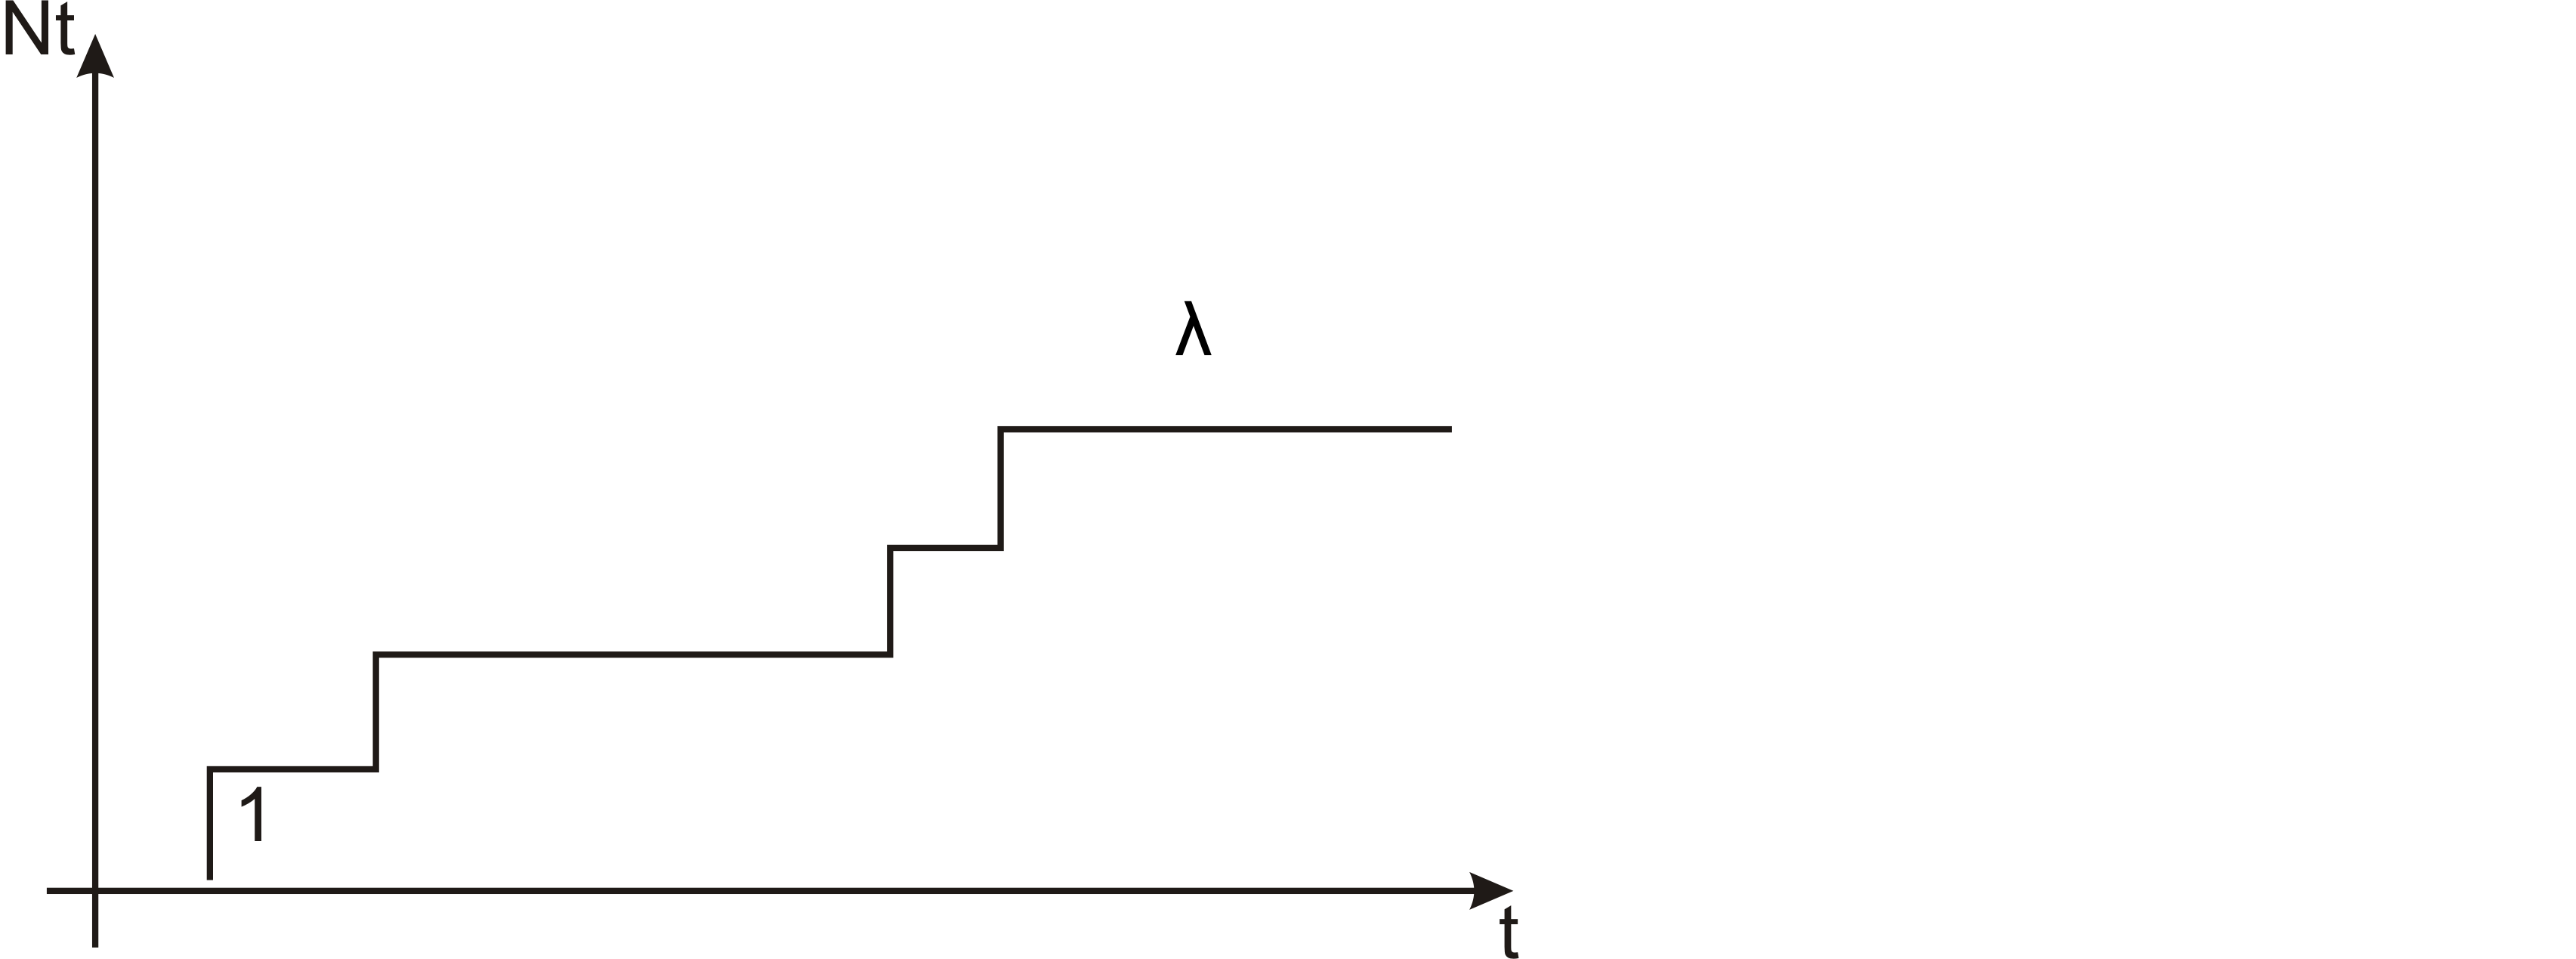
\includegraphics[width=4.5in]{Figures/rate.PNG}\\
%% \caption{}\label{}
%\end{figure}
%Suppose $\{N_{t}, t \geq 0\}$ Poisson Process with rate $\lambda$. 
%
%$\tilde{N_{t}}(w)= N_{t}(w)+f(t+X_{1}(w))$ where $f(t)$=0, if $t$ is irrational and $f(t)$=t, if $t$ is rational.\\
%\begin{eqnarray*}
%% \nonumber to remove numbering (before each align)
%P[\tilde{N_{t}}\neq N_{t}] &= P[\omega:t+X_{1}(\omega) \text{is rational}],\\
%&= P[\omega:X_1(\omega)  \text{is rational} ] =0.
%\end{eqnarray*}


\section{Non-stationary Poisson Process}
From the characterization of Poisson process just stated, we can generalize to non-homogeneous Poisson Process. 
In this case, the rate of Poisson Process $\lambda$ is time varying. 
%It is not clear from the first two characterizations, how to generalize the definition of Poisson process to the non-homogeneous case. 
%We used third characterization of Poisson process for this generalization. 

An integer valued counting process $\{N(t),~t\geqslant 0\}$ is said to be possibly \textbf{non-stationary Poisson process} if it has unit jumps and independent increments. 
That is,
\begin{enumerate} 
\item for each $\omega \in \Omega$, the map $t \mapsto N_t(\omega)$ has jumps of unit size only,
\item for any $t,s \geq 0$, the random variable $N_{t+s} - N_t$ is independent of the past $\{N_u, u \leqslant t\}$. 
\end{enumerate}
	
Let $m(t) = \E N_t$ for all $t \geqslant 0$. 
From non-decreasing property of counting processes, it follows that the mean is also non-decreasing in time $t$. 
From right continuity of counting process and the monotone convergence theorem, it follows that mean function is also right continuous. 
The \textbf{time inverse} of mean is defined as
\begin{align*}
\tau(t) &= \inf\{ s > 0 : m(s) > t\},~ t \geqslant 0. 
\end{align*}
Since, inverse of a non-decreasing function is also non-decreasing, we conclude that $\tau(t)$ is non-decreasing function of time $t$. 

\begin{thm} 
Let $N_t$ be a non-stationary Poisson process, such that $m(t) = \E N_t$ is continuous. 
Then, 
\begin{align*}
M_t(\omega) \triangleq N_{\tau(t)}(\omega),~~t \geqslant 0, \omega \in \Omega, 
\end{align*}
is a stationary Poisson process with unit rate. 
\end{thm}
\begin{proof}
Fix $t > s \geq 0$ and let $s' \triangleq \tau(s)$ and $t' \triangleq \tau(t) - \tau(s)$.  
Then, by definition of $M_t, t', s'$ and independent increment property of non-stationary Poisson process $N_t$, we have 
\begin{align*}
\E[M_{t}-M_s | M_u; u \leqslant s] &= \E[N_{t'}-N_{s'} | N_u; u \leqslant s'] = m(t') - m(s') = m(\tau(t)) - m(\tau(s)) = t-s.
\end{align*}
It follows that $M_t$ is a simple counting process with independent and stationary increments and unit rate.  
\end{proof}
\begin{cor}
Let $m(t)$ be a continuous non-decreasing function. 
Then, $S_1, S_2, \dots$ are the arrival instants in a non-stationary Poisson process $N_t$ with mean function $m(t) = \E N_t$ iff $m(S_1), m(S_2), \dots$ are the arrivals instants of a stationary Poisson process of unit rate.
\end{cor}
\begin{proof}
We can write the $n$th arrival instant  $S'_n$ of unit-rate stationary Poisson process $M_t$, in terms of the $n$th arrival instant $S_n$ of non-stationary Poisson process $N_t$ as
\begin{align*}
S'_n &= \inf\{t > 0: {\tau(t)} > S_n\} = \inf\{ t > 0: m(S_n) > t\} = m(S_n).
\end{align*}
\end{proof}
This corollary implies that $S_n \in [s,t)$ if and only if $m(S_n) \in [m(s), m(t))$. 
Therefore, number of arrivals in $[s,t)$ equals number of arrivals for unit-rate stationary Poisson process in $[m(s), m(t))$. 
Hence, we conclude that for $b(s,t) = m(t) - m(s)$
\begin{align*}
\Pr\{N_{t}-N_s = k\} &= e^{-b(s,t)}\frac{b(s,t)^k}{k!},~k \in \N_0.
\end{align*}
We will see that the inter-arrival times for the non-stationary Poisson process $N_t$, defined as
\begin{xalignat*}{3}
&T_0 = 0, &&T_n = S_n - S_{n-1},~n \in \N,
\end{xalignat*}
are not independent anymore. 
\begin{prop} 
For a non-stationary Poisson process with continuous mean function $m(t)$, we have
\begin{align*}
\Pr\{T_{n+1} > t|S_1, S_2, \dots, S_n\} &= \exp\left(-m(S_n+t) + m(S_n)\right).
\end{align*}
\end{prop}
\begin{proof}
We define events $A = \{m(S_{n+1}) > m(S_n+t)\}$ and $B = \{m(S_{n+1}) \geq m(S_n+t)\}$. 
Then, we have 
%\begin{align*}
$A \subseteq \{T_{n+1} > t\} \subseteq B$.
%\end{align*}
Hence, we can write 
\begin{align*}
\Pr\{A|S_1, S_2, \dots, S_n\} &\leq \Pr\{T_{n+1} > t |S_1, S_2,\dots, S_n\}.
\end{align*}
The arrival instants $S_1, \dots, S_n$ determine $m(S_1), \dots, m(S_n), m(S_n+t)$. 
Further, since $m(S_{n+1}) - m(S_n)$ is the inter-arrival time of the stationary Poisson process $M(t)$, 
it is independent of $S_1,S_2,\dots, S_n$
\begin{align*}
\Pr\{A|S_1,\dots, S_n\} &= \Pr\{m(S_{n+1})-m(S_n) > m(S_n+t) - m(S_n) |S_1,\dots,S_n\} = \exp\left(-m(S_{n}+t)+m(S_n)\right).
\end{align*}
Result follows from the continuity of the exponential distribution. 
\end{proof}

\section{Laplace Functional}
The \textbf{Laplace functional} $\L$ of a point process $\Phi$ and associated counting process $N$ is defined for all non-negative function $f: \R^d \to \R$ as 
\begin{align*}
\L_{\Phi}(f) &= \E \exp\left(-\int_{\R^d}f(x)N(dx)\right).
\end{align*}
For simple function $f(x) = \sum_{i = 1}^{k}t_i1\{x \in A_i\}$, we can write the Laplace functional 
\begin{align*}
\L_{\Phi}(f) &= \E\exp(-\sum_{i}t_iN(A_i)),
\end{align*}
as a function of the vector $(t_1, t_2, \dots, t_k)$, a joint Laplace transform of the random vector $(N(A_1), \dots, N(A_k))$. 
This way, one can compute all finite dimensional distribution of the counting process $N$. 
\begin{prop}
The Laplace functional of the Poisson process with intensity measure $\Lambda$ is 
\begin{align*}
\L_{\Phi}(f) &= \exp\left(-\int_{\R^d}(1-e^{-f(x)})\Lambda(dx)\right).
\end{align*}  
\end{prop}
\begin{proof}
For a bounded Borel measurable set $A \subseteq \R^d$, consider $g(x) = f(x)1\{x \in A\}$. 
Then,
\begin{align*}
\L_{\Phi}(g) &= e^{-\Lambda(A)}\sum\exp\left(-\int_{\R^d}(1-e^{-f(x)})\Lambda(dx)\right).
\end{align*}  
\end{proof}


\end{document}


%\begin{defn}[Non-Homogeneous Poisson Process]\label{defn:NonHomogeneousPoisson} 
A point Process $\{N(t),~t\geqslant 0\}$ is said to be \textbf{nonhomogeneous Poisson Process} with instantaneous rate $m(t)$ if it has stationary independent increments, and 
	\begin{eqnarray*}\label{eq:NonHomogeneousPoisson}
		\Pr\{N(t)=0\}&=&1-m(t)+o(t). \\
		\Pr\{N(t+\delta)-N(t)=0\} &=& 1-m(t)\delta+o(\delta). \\
		\Pr\{N(t+\delta)-N(t)=1\} &=& m(t)\delta+o(\delta). \\
		\Pr\{N(t+\delta)-N(t)>1\} &=& o(\delta). \\
	\end{eqnarray*}
%\end{defn}

\begin{prop}[Non-Homogeneous Distribution] Distribution of non-homogeneous Poisson Process $N(t)$ with instantaneous rate $m(t)$ is given by
	\begin{align*}
		\Pr\{N(t)=n\}=\frac{(\bar{m}(t))^n}{n!}e^{-\bar{m}(t)},
	\end{align*}
	where $\bar{m}(t)$ is the cumulative rate till time $t$, i.e. $\bar{m}(t)=\int_{0}^{t}m(s)ds$. 
\end{prop}
\begin{proof}
	Let's denote $f(t) = \Pr\{N(t)=0\}$. Further, from independent increment property of $N(t)$, we notice that $\{N(t+\delta) = 0\}$ is intersection of two independent events given below, 
	\begin{align*}
		\{N(t+\delta)=0\} \iff \{N(t)=0\}\cap\{N(t+\delta)-N(t)=0\}.
	\end{align*}
	From Definition~\ref{defn:NonHomogeneousPoisson}, it follows that
	\begin{align*}
		f(t+\delta) = f(t)[1 - m(t)\delta + o(\delta)].
	\end{align*}
	Re-arranging the terms in the above align, dividing by $\delta$, and taking limit as $\delta \downarrow 0$, we get 
	\begin{align*}
		f'(t) = -m(t)f(t).
	\end{align*}
	Since $f(0) = 1$, it can be verified that $f(t) = \exp(-\bar{m}(t))$ is solution for $f(t)$.
	%\begin{eqnarray*}
	%f(t+\triangle) &=& \Pr\{N_{t+\triangle}=0] \\
	%&=&  \Pr\{N(t)=0, N_{t+\triangle}-N(t)=0]\\
	%&\stackrel{(a)}{=}& \Pr\{N(t)=0] \Pr\{N_{t+\triangle}-N(t)=0]\\
	%&=& f(t)[1-m(t)\triangle +o(\triangle)].\\
	%\frac{f(t+\triangle)-f(t)}{\triangle} &=& -m(t) f(t) +f(t) \frac{0(\triangle)}{\triangle}. \\
	%\lim_{\triangle\downarrow 0}\frac{f(t+\triangle)-f(t)}{\triangle} &=& -m(t) f(t) \\
	%\frac{d f(t)}{t} &=& -m(t) f(t),  \\
	%\end{eqnarray*}
	%where (a) follows from independent increment property. Since, $\overline{m}(t)=\int ^{t}_{0} m(s) ds $, $f(t)=\Pr\{N(t)=0]$, $ f(0)=\Pr\{N_{0}=0] =1$ the solution of the differential align can be verified to be $f(t)=e^{-\overline{m}(t)}$, as follows: 
	%\begin{eqnarray*}
	%f(0)&=& e^{-\overline{m}(t)}\\
	%&=& e^{-0}=1 \\
	%f'(t) &=& e^{-\overline{m}(t)}\frac{d}{dt} \int^{t}_{0}m(S) ds\\
	%&=& m(t)e^{-\overline{m}(t)}, t\geqslant 0 \\
	%\end{eqnarray*}
	%
	%\begin{eqnarray*}
	%\Pr\{N_{t+\triangle}-N(t)=0] &=& 1-m(t)\triangle +o(\triangle) \\
	%\Pr\{N_{\triangle}-N_{0}=0] &=& 1-m(0)\triangle +o(\triangle) 
	%\end{eqnarray*}
	%Since $ N_{0}=0$, 
	%\begin{eqnarray*}
	%\Pr\{N_{\triangle} =0]&=& 1-m(0)\triangle +0(\triangle) \\
	%\lim_{\triangle\downarrow 0}f(\triangle) &=& f(0)=1.
	%\end{eqnarray*}
	We have shown $\Pr\{N(t)=0\} = \exp(-\bar{m}(t))$. By induction, we can show the result for any $n$.
\end{proof}